La struttura del progetto è organizzata in due macro package, il package \texttt{GUI}(Graphical User Interface) si occupa unicamente di gestire 
l'interfaccia utente, mentre il package \texttt{backend} contiene l'implementazione della nostra DCT2, 
la configurazione dei benchmark, la logica per la compressione delle immagini(con la DCT2 nel formato fast
offerta dalla libreria esterna \texttt{JTransform}) e la generazione dei risultati in formato CSV per i 
benchmark e immagini in formato BMP per la compressione delle immagini.
\\
La figura \ref{fig:project_structure} mostra la struttura del progetto. 
\begin{figure}[hbt]
    \centering
    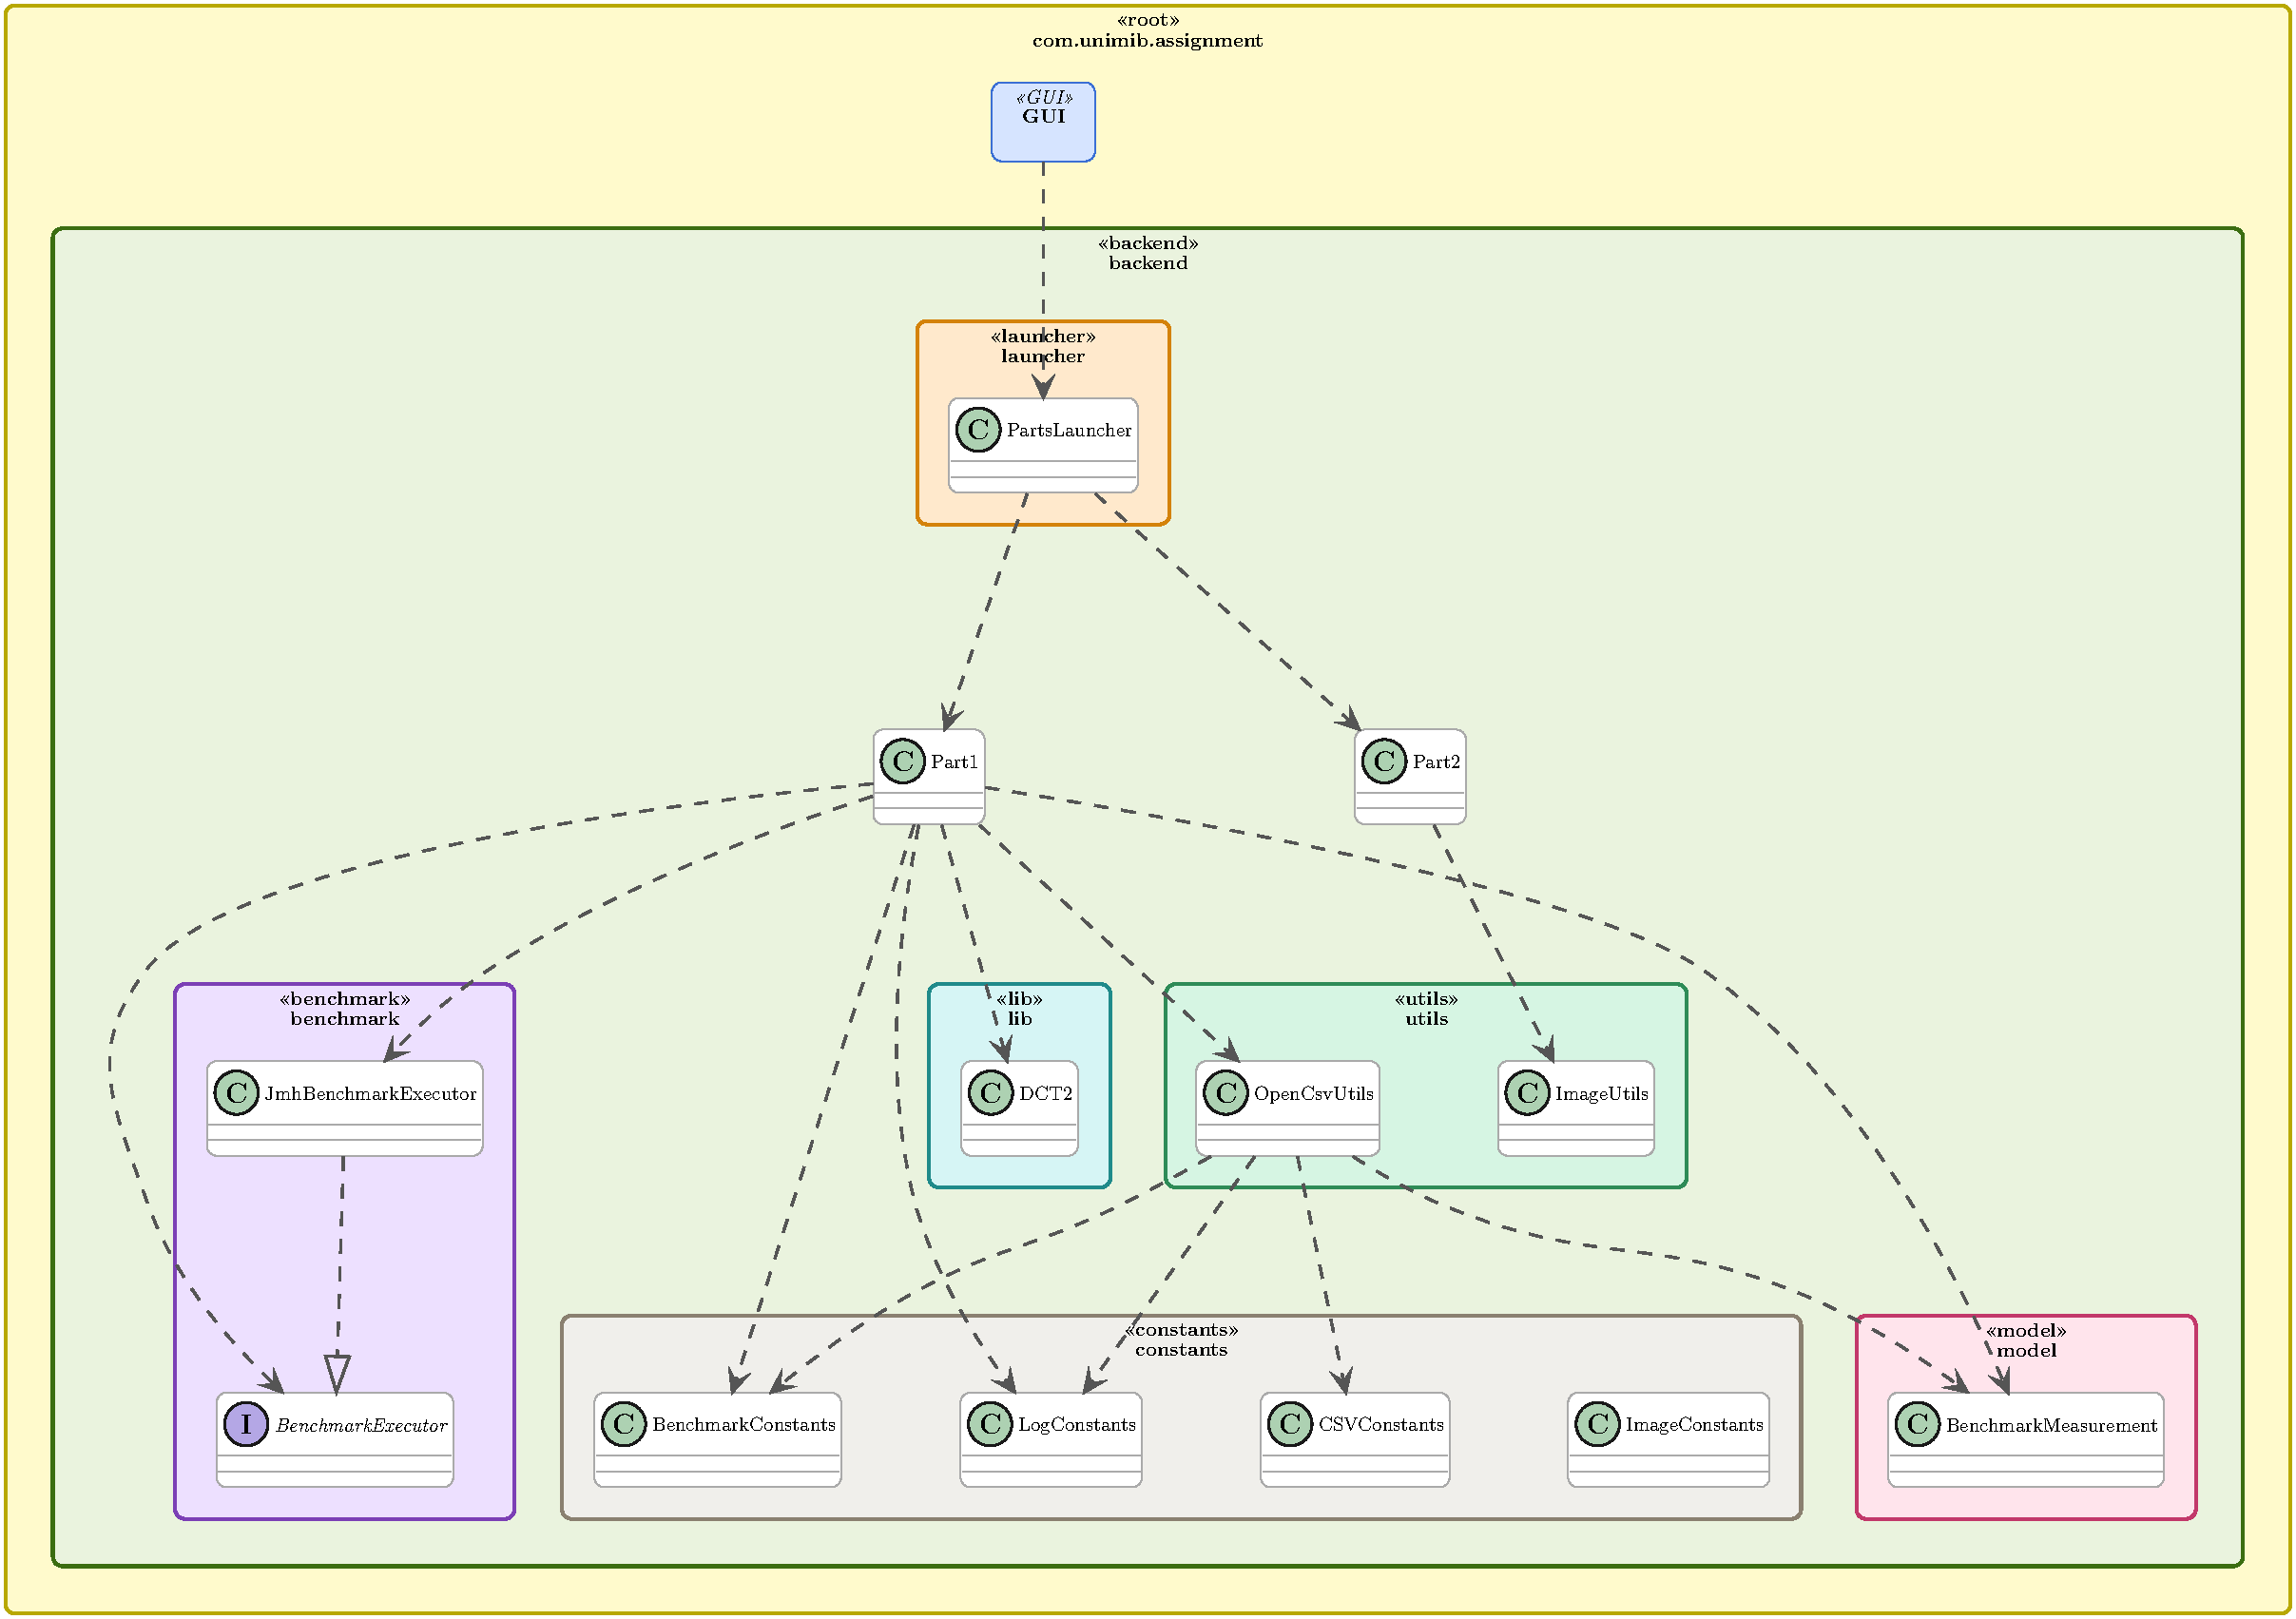
\includegraphics[width=\textwidth]{../architecture/architecture.pdf}
    \caption{Struttura del progetto}
    \label{fig:project_structure}
\end{figure}
\clearpage
\section{Implementazione della DCT2}
Il package \texttt{com.unimib.assignment.backend.lib} contiene l'implementazione della DCT2, questa classe 
implementa un metodo chiamato DCT-II che funge da algoritmo core per i due metodi offerti: 
\lstinputlisting[
	language=Java,
	style = Java,
	caption = Algoritmo DCTII(DCT2) implementato nel package \texttt{lib},
	firstline=79,
	lastline=107,
	label=ls:DCT2
]{../code/src/main/java/com/unimib/assignment/backend/lib/DCT2.java}
Questa implementazione è utilizzata sia per il metodo forward(DCT2):
 \lstinputlisting[
	language=Java,
	style = Java,
	caption = Algoritmo forward implementato nel package \texttt{lib},
	firstline=38,
	lastline=44,
	label=ls:DCT2
]{../code/src/main/java/com/unimib/assignment/backend/lib/DCT2.java}
che per il metodo inverse(IDCT2): 
\lstinputlisting[
	language=Java,
	style = Java,
	caption = Algoritmo inverse implementato nel package \texttt{lib},
	firstline=57,
	lastline=64,
	label=ls:DCT2
]{../code/src/main/java/com/unimib/assignment/backend/lib/DCT2.java}
Questo approccio ci permette di avere un codice più pulito e leggibile, 
evitando la duplicazione del codice per i due metodi.
\footnote{L'implementazione della DCT2 si appoggia alla libreria EJML, questo permette di avere
un codice più leggibile rispetto a un'implementazione basata su matrici}

\section{Part1 e Part2}

Il package \texttt{com.unimib.assignment.backend.launcher} offre la classe \texttt{PartsLauncher},
che espone alla UI due metodi: \texttt{launchAndHandlePart1}, per l'avvio dei benchmark, e
\texttt{launchPart2}, per la compressione delle immagini.

\paragraph{launchAndHandlePart1}
si occupa di invocare la classe \texttt{Part1}, responsabile della gestione del processo di esecuzione dei 
benchmark e della memorizzazione dei risultati.

Come prima operazione, richiama il metodo \texttt{randomMatrix} per generare le matrici casuali da utilizzare
nei benchmark. Tali matrici vengono create prima dell'esecuzione dei test e condivise tra il benchmark 
della nostra implementazione della DCT2 e quello della libreria, così da garantire risultati confrontabili. 
Le dimensioni delle matrici sono memorizzate nell'array di interi \texttt{BENCHMARK\_BLOCK\_SIZES}.

Per l'esecuzione dei benchmark, la classe \texttt{Part1} si occupa di:
\begin{enumerate}
\item invocare la classe \texttt{JmhBenchmarkExecutor}, responsabile della configurazione e dell'esecuzione 
dei benchmark tramite JMH. Tale classe gestisce le iterazioni di warmup 
(\texttt{DEFAULT\_WARMUP\_ITERATIONS} = 3) e quelle di misurazione 
(\texttt{DEFAULT\_MEASUREMENT\_ITERATIONS} = 5), salvando i risultati nel record 
\textsl{BenchmarkMeasurement(size, meanTimeMine, meanTimeLib)}. I tempi sono memorizzati in secondi;
\item salvare i risultati contenuti nel record \textsl{BenchmarkMeasurement} in un file CSV utilizzando la c
lasse \texttt{OpenCsvUtils}, che si appoggia alla libreria opensource \texttt{OpenCSV} \cite{opencsv};
\item gestire eventuali richieste di terminazione forzata del benchmark provenienti dalla UI, 
interrompendone l'esecuzione.
\end{enumerate}

\paragraph{launchPart2}
Si occupa di eseguire la compressione delle immagini utilizzando la trasformata DCT2 fornita dalla libreria
\texttt{JTransform}, di inviare l'immagine compressa alla UI e di salvare le immagini compresse in formato BMP.

La classe \texttt{Part2} contiene i seguenti metodi:

\begin{itemize}
    \item \texttt{BufferedImage compress(Pair<String, BufferedImage> imageInfo, int F, int d)}: esegue l'intera pipeline di compressione dell'immagine:
    \begin{enumerate}
        \item converte l'immagine di input in una matrice di \texttt{double};
        \item ritaglia la matrice in modo che le sue dimensioni siano multipli di \texttt{F};
        \item per ogni blocco di dimensione \texttt{F} $\times$ \texttt{F}, richiama il metodo \texttt{compressBlock} per effettuare la compressione;
        \item converte la matrice risultante in una \texttt{BufferedImage};
        \item salva l'immagine compressa nella cartella \texttt{output} e successivamente la inoltra alla UI.
    \end{enumerate}

    \item \texttt{void compressBlock(double[][] signal, int i, int j, int F, int d)}: comprime un blocco dell'immagine di dimensione \texttt{F} $\times$ \texttt{F}:
    \begin{enumerate}
        \item copia il blocco in una matrice di \texttt{double};
        \item applica la DCT2 al blocco utilizzando il metodo \texttt{forward(matrix, scale)} dell'oggetto \texttt{DoubleDCT\_2D} della libreria \texttt{JTransform}, impostando \texttt{scale = true}. In questo modo viene utilizzata una normalizzazione ortonormale, coerente con quella adottata nella nostra implementazione della DCT2;
        \item elimina le componenti ad alta frequenza in base al parametro \texttt{d};
        \item applica la trasformata inversa IDCT2 mediante il metodo \texttt{inverse(matrix, scale)}, con \texttt{scale = true};
        \item richiama il metodo \texttt{shiftBlockBy255} per riportare i valori del blocco nell'intervallo \([0, 255]\);
        \item copia il blocco compresso nella matrice dell'immagine risultante.
    \end{enumerate}

    \item \texttt{void shiftBlockBy255(double[][] matrix)}: effettua uno shift dei valori nell'intervallo \([0, 255]\), riportandoli nel dominio delle immagini BMP.
\end{itemize}

I metodi di conversione tra \texttt{BufferedImage} e matrici di \texttt{double} e il salvataggio
in formato BMP sono implementati nella classe \texttt{ImageUtils}.

\subsection{GUI}
Il package \texttt{com.unimib.assignment.GUI} offre 3 schermate principali: due schermate iniziali per il lancio dei benchmark
e per l'avvio della compressione delle immagini, una schermata dedicata alla compressione e una schermata per
l'inserimento dei parametri di compressione. La Figura \ref{fig:main-screen-1} mostra la schermata iniziale per la scelta tra benchmark e compressione,
la Figura \ref{fig:main-screen-2} la schermata iniziale una volta scelta l'opzione benchmark, la Figura \ref{fig:compression-screen}
la schermata di compressione delle immagini e la Figura \ref{fig:parameters-screen} la schermata d'inserimento dei parametri di compressione.
Per l'avvio dei benchmark e della compressione delle immagini, la UI si appoggia alla classe 
\texttt{PartsLauncher} del package \texttt{backend.launcher}.
\begin{figure}[hbt]
    \centering
    \begin{minipage}[t]{0.44\textwidth}
        \centering
        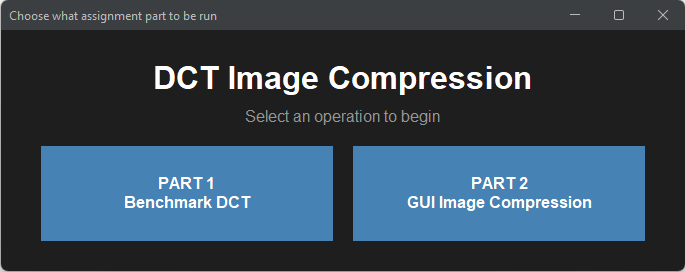
\includegraphics[width=\linewidth]{figures/main-screen-1.png}

        \small Schermata iniziale per la scelta tra benchmark e compressione delle immagini
        \label{fig:main-screen-1}
    \end{minipage}\hfill
    \begin{minipage}[t]{0.44\textwidth}
        \centering
        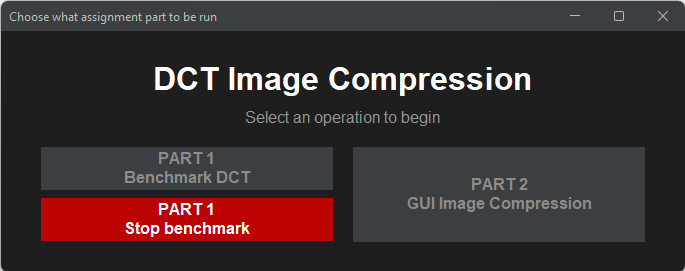
\includegraphics[width=\linewidth]{figures/main-screen-2.png}

        \small Schermata iniziale una volta scelta l'opzione di benchmark
        \label{fig:main-screen-2}
    \end{minipage}
\end{figure}

\begin{figure}[hbt]
    \centering
    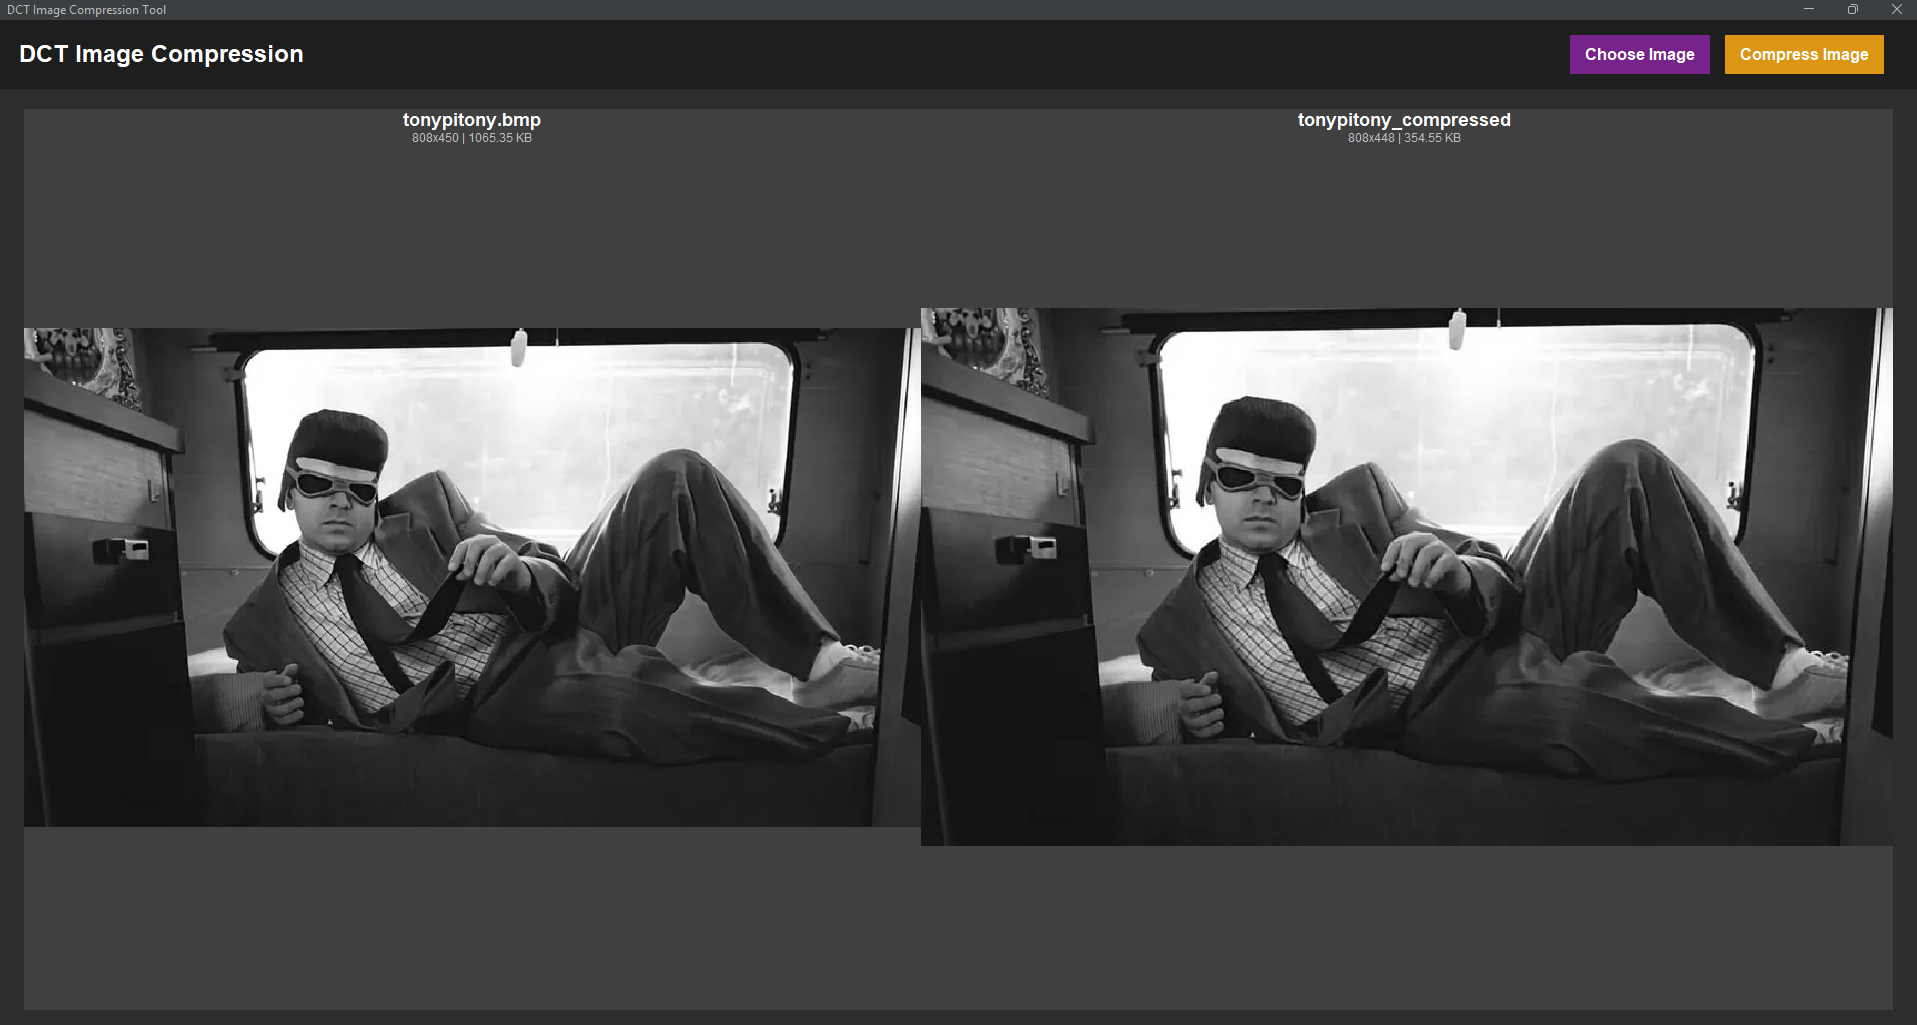
\includegraphics[width=\textwidth]{figures/compression-screen.png}
    \caption{Schermata di compressione delle immagini}
    \label{fig:compression-screen}
\end{figure}

\begin{figure}[hbt]
    \centering
    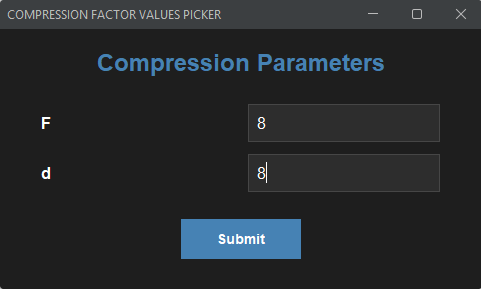
\includegraphics[width=0.35\textwidth]{figures/parameters-screen.png}
    \caption{Schermata d'inserimento dei parametri di compressione}
    \label{fig:parameters-screen}
\end{figure}
